\documentclass{beamer}
\usetheme{Berlin}
%\usecolortheme{beetle}
\title{Case Studies - Forecasting Bitcoin: \\Data Presentation}
\author{Elchin \textbf {Babayev}\\
Mert \textbf{Basaran}\\
Alkim Can \textbf{Celik}\\
Halil Anil \textbf{Demirbas}\\
Deniz \textbf{Uygur}}
\institute{Technische Universität Dortmund}
\date{18/04/2023}
\usepackage{tikz}
\begin{document}
	\begin{frame}
		\titlepage % beamer's \maketitle
	\end{frame}
	\section{Introduction}
	\begin{frame}
		\frametitle{Introduction}
		\begin{itemize}
			\item Project Context: Forecasting the quarterly growh rate of the Bitcoin.
			\item Potential Drivers: US unemployment rate, the US inflation rate, the federal funds rate and the growth rate of the S\&P 500
			\item *
		\end{itemize}
	\end{frame}
	\section{Data}
	\subsection{Data Recruitment}
		\begin{frame}
		\frametitle{Data}
		\framesubtitle{Data Recruitment}
			\begin{columns}
				\begin{column}{0.5\textwidth}
					\textbf{Historical Bitcoin Data}
					\begin{itemize}
						\item \emph {Investing.com}
						\item One of the top three global financial websites in the world.
					\end{itemize}
				\end{column}
				\begin{column}{0.5\textwidth}
					\textbf{Other Drivers}
				\begin{itemize}
					\item \emph{FRED-QD}
					\item It is a large macroeconomic database designed for the empirical analysis of “big data.”
				\end{itemize}
				\end{column}
		\end{columns}
	\end{frame}
	\subsection{Dataset Properties}	
	\begin{frame}
	\frametitle{Data}
		\framesubtitle{Dataset Properties}
		\begin{columns}
				\begin{column}{0.5\textwidth}
					\textbf{Historical Bitcoin Data}
					\begin{itemize}
						\item \emph{.csv} format
						\item Starts from Q3 2010
						\item Runs daily, over 4650 data points and counting
						\item 7 columns in total namely: \emph{Date, Price, Open, High, Low, Volume, Change \%}
					\end{itemize}
				\end{column}
				\begin{column}{0.5\textwidth}
					\textbf{Other Drivers}
				\begin{itemize}
					\item \emph{.csv} format
					\item Starts from Q1 1959
					\item Runs \emph{quarterly,} over 200 individual columns
				\end{itemize}
				\end{column}
		\end{columns}
	\end{frame}
	\subsection{Data Operations}	
	\begin{frame}
	\frametitle{Data}
		\framesubtitle{Data Operations}
					\textbf{Historical Bitcoin Data}
					\begin{itemize}
						\item Added a column called \emph{change,} according to the growth rate formula
						\item Fixed the \emph{volume} column which had \emph{K, M, B} corresponding to thousand, million and billion.
						\item Changed the time index to be readible by R.
						\item Daily data has been aggregated to be quarterly data using averages over the given period.
					\end{itemize}
	\end{frame}
	\begin{frame}
		\textbf{Other Drivers}
			\begin{itemize}
			\item In total of 8 columns have been used, namely \emph{UNRATE','CPIAUCSL', 'CPILFESL', 'FEDFUNDS', 'S.P.500', 'S.P..indust', 'S.P.div.yield'}
			\end{itemize}
		{\scriptsize
		\begin{tabular}{|l|l|} \hline
			Column & Description \\ \hline
			UNRATE & Civilian Unemployment Rate (Percent) \\ 
			CPIAUCSL & CPI for All Urban Consumers: All Items \\
			CPILFESL & CPI for All Urban Consumers: All Items Less Food Energy \\
			FEDFUNDS & Effective Federal Funds Rate\\
			S.P.500 & S\&P’s Common Stock Price Index: Composite\\
			S.P..indust & S\&P’s Common Stock Price Index: Industrials\\
			S.P.div.yield & S\&P’s Composite Common Stock: Dividend Yield\\ \hline
		\end{tabular}}		
	\end{frame}
	\begin{frame}
		\textbf{Other Drivers}
		\begin{itemize}
			\item Created data for \emph{infilation} from the CPI
			\item Derived the growth rate for S\&P indexes
		\end{itemize}
		All of the variables have been combined in a dataframe called \emph{combined\_df}
	\end{frame}
	\subsection{Data Visualisations}
	\begin{frame}
	\frametitle{Data}
	\framesubtitle{Data Visualisations}
		\begin{figure}
			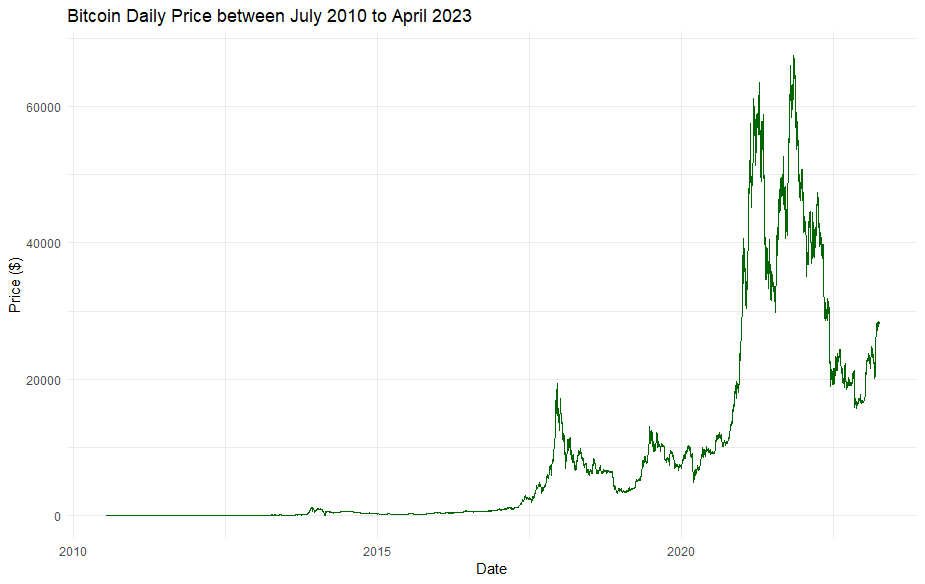
\includegraphics[
			width=0.75\textwidth]{BTC_Daily_all}
			\caption{Historical Bitcoin Price Data}
			\label{fig:BTCall}
		\end{figure}
	\end{frame}
	\begin{frame}
	\textbf{Descriptive Statistics for Historical Daily Bitcoin Price}
		\begin{tabular}{|c|c|} \hline
			Metric & Value \\ \hline
			Data Points & 4644 \\ 
			Mean & 8,894.42 \\
			Standard Deviation & 14,497.53 \\
			Median & 902.65\\
			Minimum & 0.1\\
			Maximum & 67,527.9\\ \hline
		\end{tabular}
		\end{frame}
	\begin{frame}
	\begin{figure}
			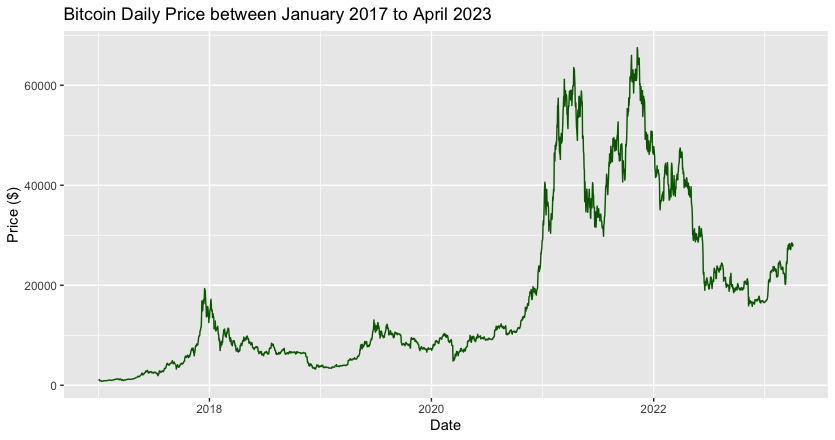
\includegraphics[
			width=0.75\textwidth]{BTC_Daily_2017}
			\caption{Historical Bitcoin Price Data 2017-2023}
			\label{fig:BTCpart}
		\end{figure}
	\end{frame}
	
	\begin{frame}
	\begin{figure}
			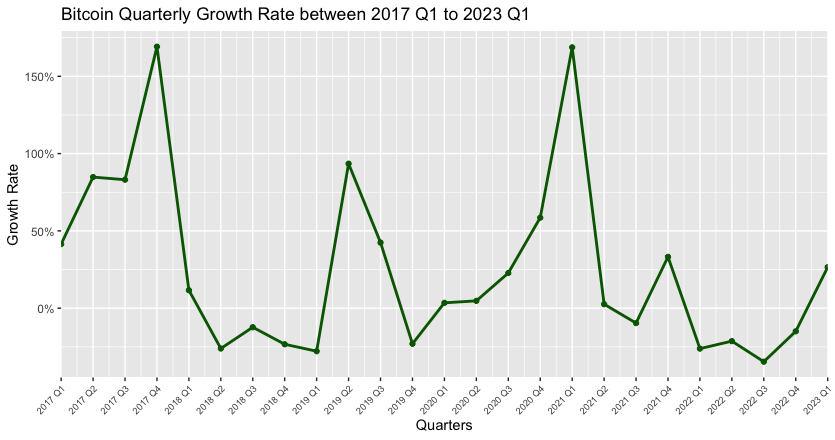
\includegraphics[
			width=0.75\textwidth]{BTC_Growth_2017}
			\caption{Historical Quarterly Bitcoin Price Growth 2017-2023}
			\label{fig:BTCpart1}
		\end{figure}
	\end{frame}
	
	\begin{frame}
	\begin{figure}
			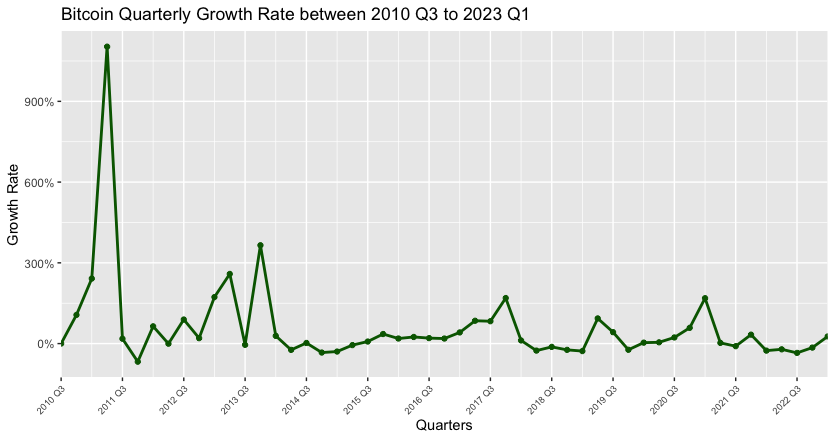
\includegraphics[
			width=0.75\textwidth]{BTC_G_All}
			\caption{Historical Quarterly Bitcoin Price Growth 2010-2023}
			\label{fig:BTCpart1}
		\end{figure}
	\end{frame}
	%\begin{frame}
	%\begin{figure}
	%		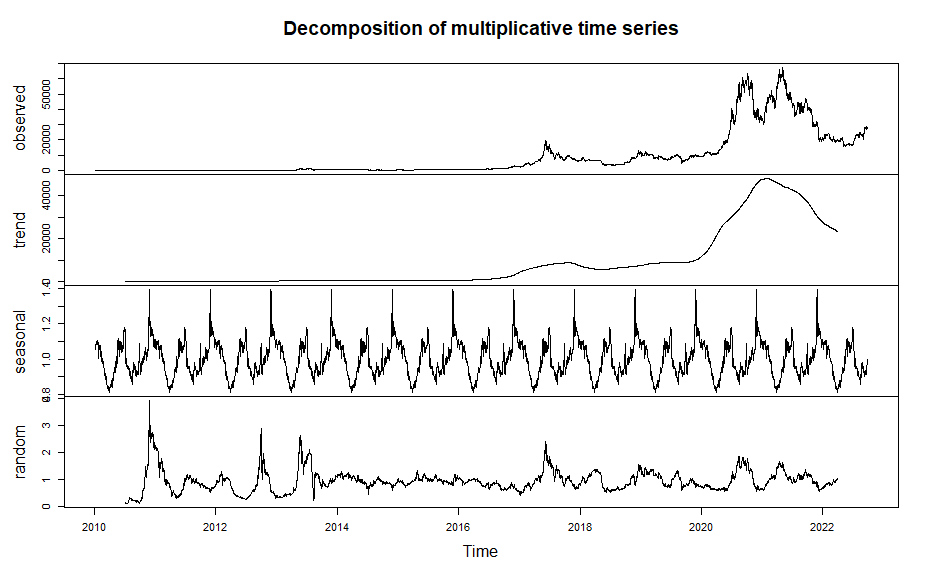
\includegraphics[
	%		width=0.75\textwidth]{BTC_Daily_Decomposition}
	%		\caption{BTC Daily Decomposition}
	%		\label{fig:BTCdecomp}
	%	\end{figure}
	%\end{frame}
	\begin{frame}
	\begin{figure}
			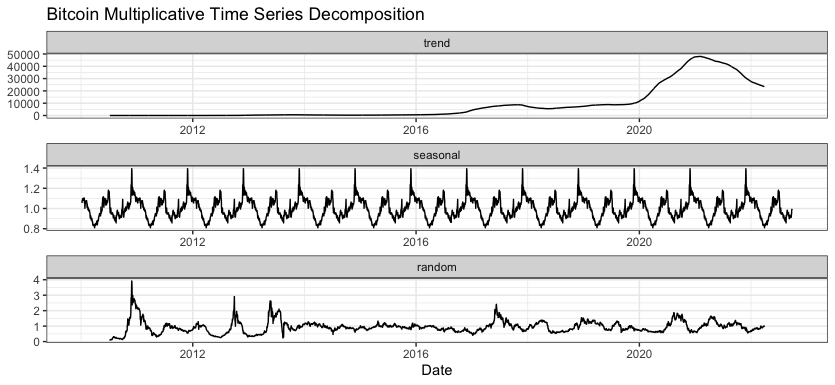
\includegraphics[
			width=1\textwidth]{BTC_decom}
			\caption{BTC Daily Decomposition}
			\label{fig:BTCdecomp}
		\end{figure}
	\end{frame}




	
	       
        \begin{frame}
	\begin{figure}
			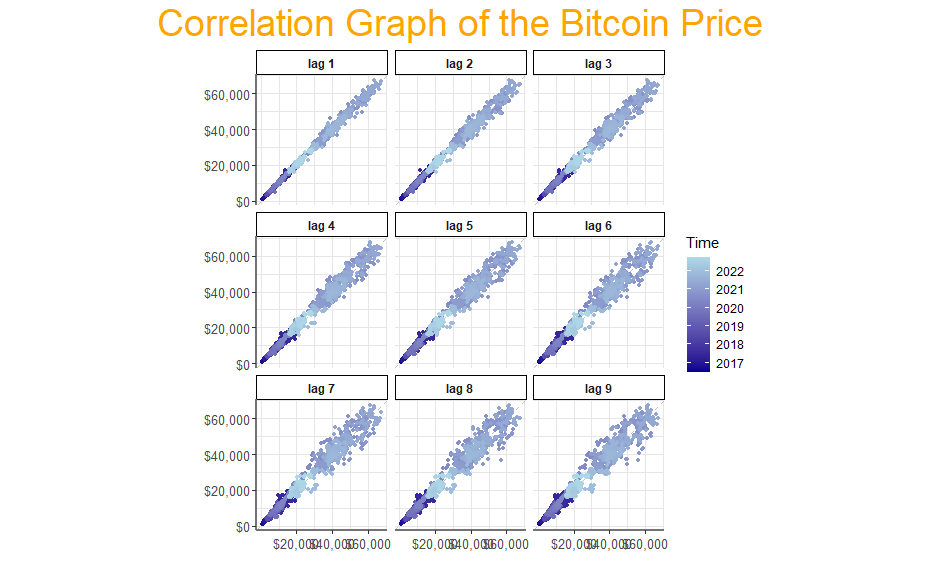
\includegraphics[
			width=0.75\textwidth]{BTC_lag_corr}
			\caption{BTC Lagged correlations}
			\label{fig:BTCcorr}
		\end{figure}
	\end{frame}
	\begin{frame}
	\begin{figure}
			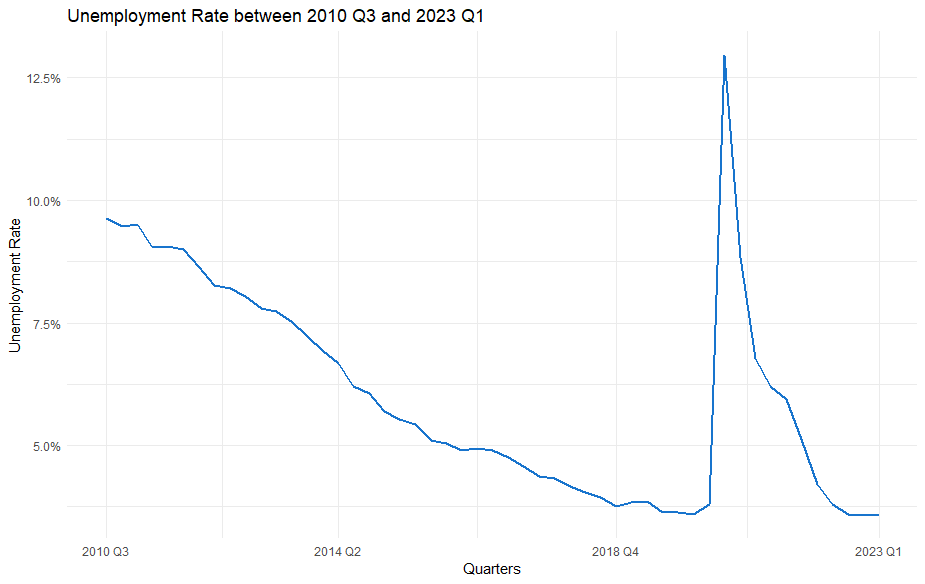
\includegraphics[
			width=0.75\textwidth]{Unemployment}
			\caption{Quarterly Unemployment}
			\label{fig:Unemp}
		\end{figure}
	\end{frame}
	\begin{frame}
	\begin{figure}
			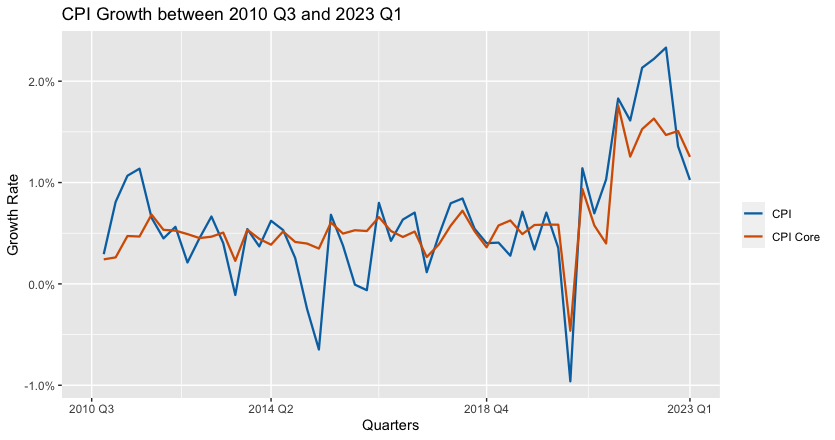
\includegraphics[
			width=0.75\textwidth]{CPI_Growth}
			\caption{CPI Growth Rate}
			\label{fig:Inf}
		\end{figure}
	\end{frame}
	\begin{frame}
	\begin{figure}
			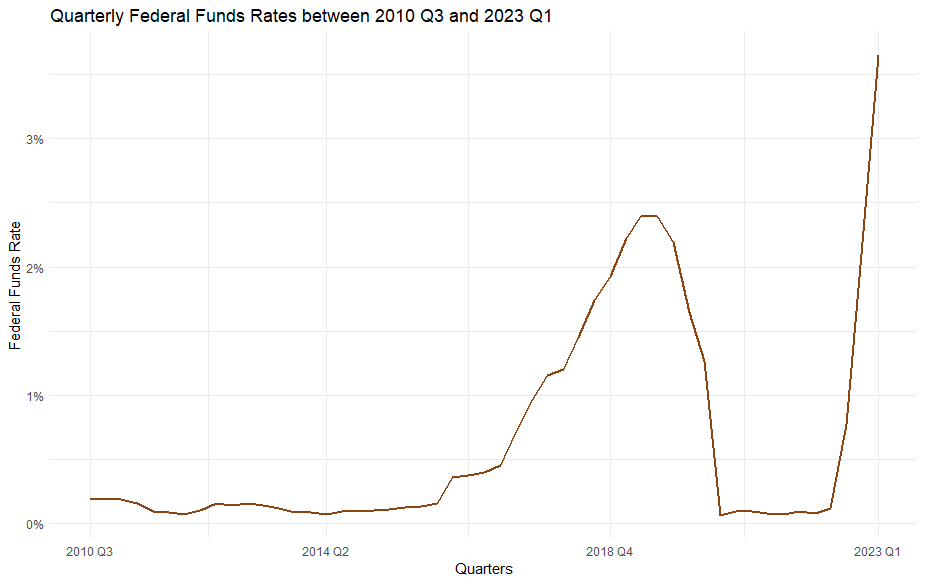
\includegraphics[
			width=0.75\textwidth]{Federal_Funds_Rate}
			\caption{Federal Funds Rate}
			\label{fig:FED}
		\end{figure}
	\end{frame}
	\begin{frame}
	\begin{figure}
			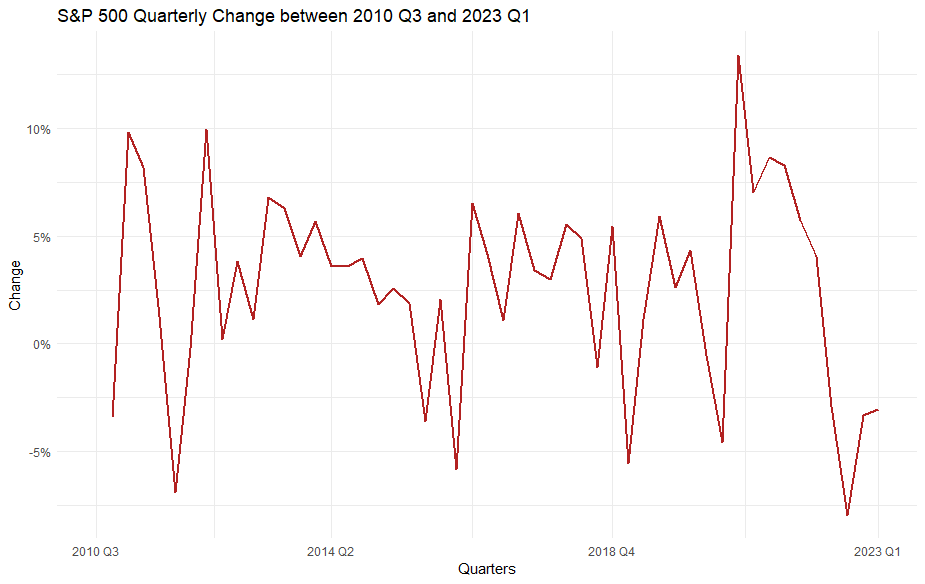
\includegraphics[
			width=0.75\textwidth]{S&P_Quarterly}
			\caption{Quarterly S\&P}
			\label{fig:sP}
		\end{figure}
	\end{frame}
	\begin{frame}
	\begin{figure}
			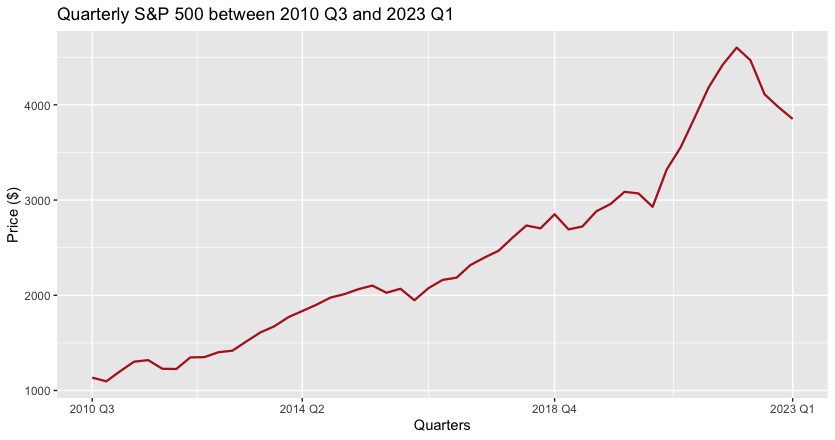
\includegraphics[
			width=0.75\textwidth]{SP_Price}
			\caption{Quarterly S\&P Price}
			\label{fig:sPP}
		\end{figure}
	\end{frame}
		\begin{frame}
	\begin{figure}
			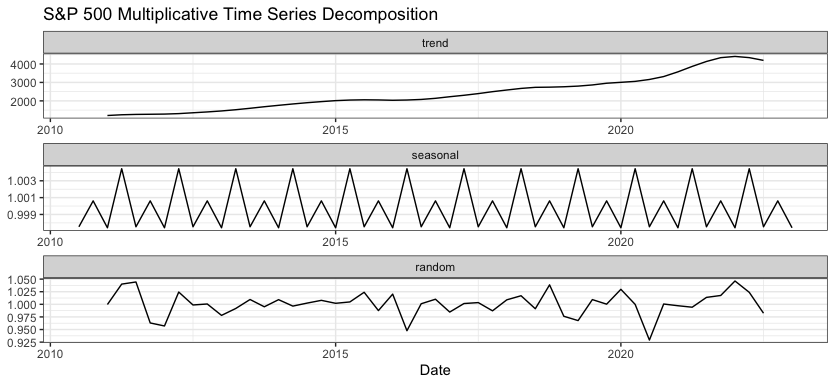
\includegraphics[
			width=0.75\textwidth]{SP_decom}
			\caption{S\&P 500 Decomposition }
			\label{fig:sPPP}
		\end{figure}
	\end{frame}

	
	
	\begin{frame}
		\begin{block}{Interesting Fact}
			This is important.
		\end{block}
		\begin{alertblock}{Cautionary Tale}
			This is really important!
		\end{alertblock}
	\end{frame}
	\begin{frame}
	\begin{figure}
			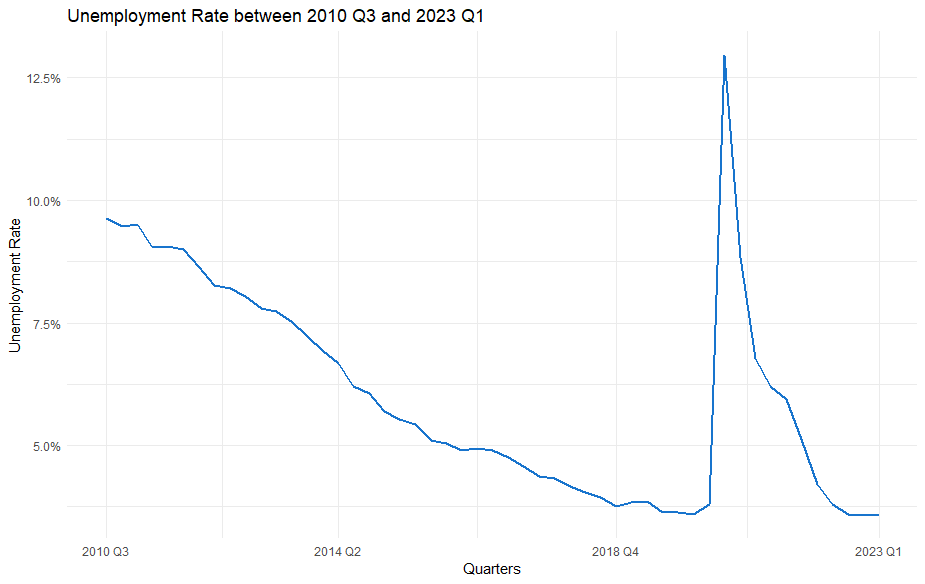
\includegraphics[
			width=0.75\textwidth]{Unemployment}
			\caption{Quarterly Unemployment}
			\label{fig:Unemp}
		\end{figure}
	\end{frame}
         \begin{frame}
	\begin{figure}
			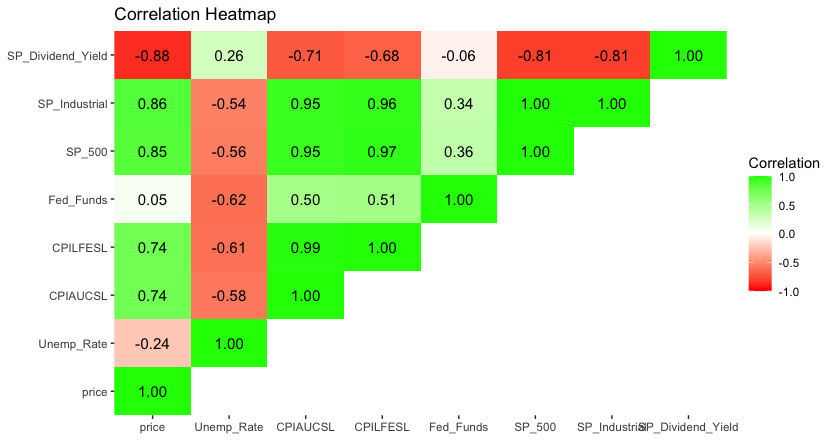
\includegraphics[
			width=0.75\textwidth]{Correlation_HM}
			\caption{Correlation Heat Map}
			\label{fig:Correlation All}
		\end{figure}
	\end{frame}

\end{document}